% This is samplepaper.tex, a sample chapter demonstrating the
% LLNCS macro package for Springer Computer Science proceedings;
% Version 2.20 of 2017/10/04
%
\documentclass{llncs}
%
\usepackage{graphicx}
% Used for displaying a sample figure. If possible, figure files should
% be included in EPS format.
%
% If you use the hyperref package, please uncomment the following line
% to display URLs in blue roman font according to Springer's eBook style:
% \renewcommand\UrlFont{\color{blue}\rmfamily}

\begin{document}
%
\title{A Short Instruction for \sf{nnbarrier}}
%
%\titlerunning{Abbreviated paper title}
% If the paper title is too long for the running head, you can set
% an abbreviated paper title here
%
\author{Hengjun Zhao}

\institute{School of Computer and Information Science\\
Southwest University, Chongqing, 400715, P.~R.~China\\
\email{zhaohj2016@swu.edu.cn}}
%
\maketitle % typeset the header of the contribution
%
% \begin{abstract}
% To be completed
% %\keywords{First keyword  \and Second keyword \and Another keyword.}
% \end{abstract}
%
%
\section{Introduction}
\subsection{A Subsection Sample}

Please \cite{Prajna04safetyverification} try to avoid rasterized images for line-art diagrams and
schemas. Whenever possible, use vector graphics instead (see
Fig.~\ref{fig1}).

\begin{figure}
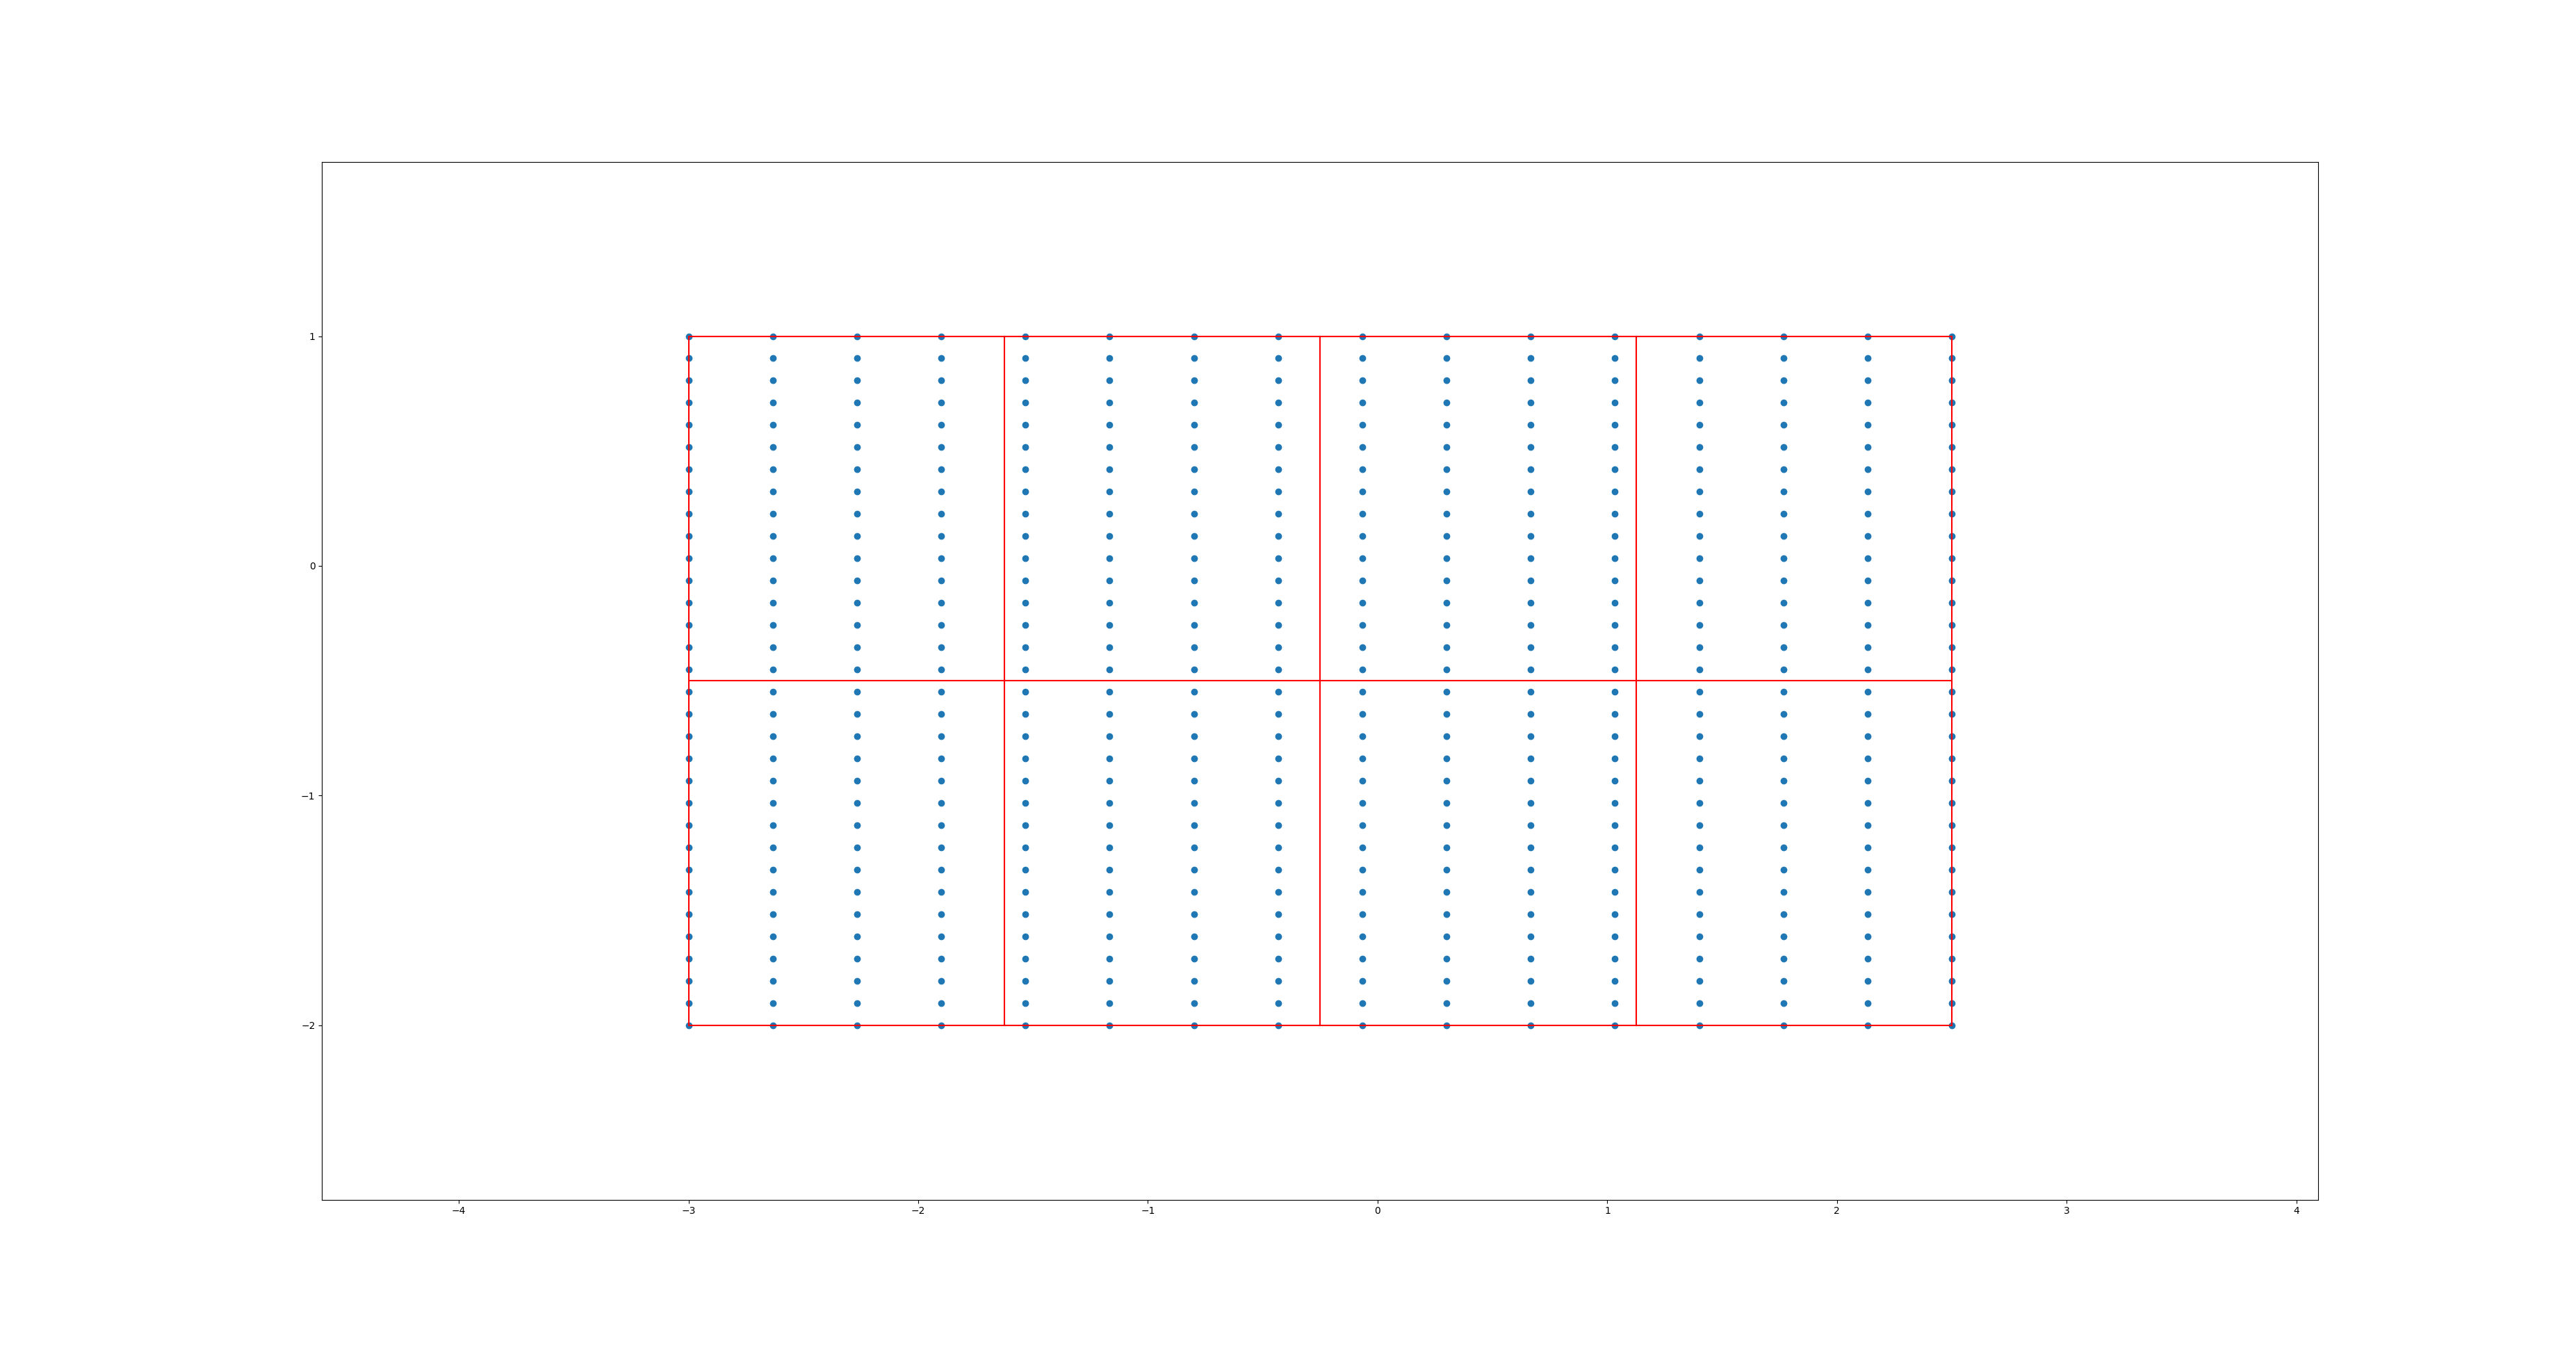
\includegraphics[width=\textwidth]{./fig/batch_data}
\caption{A figure caption is always placed below the illustration.
Please note that short captions are centered, while long ones are
justified by the macro package automatically.} \label{fig1}
\end{figure}

\section{Installation}

\section{Sample Input}

\section{Cases in the Paper}

\section{Define Your Own Problem}


\bibliographystyle{splncs04}
\bibliography{instruction}

% \begin{thebibliography}{8}
% \bibitem{ref_article1}
% Author, F.: Article title. Journal \textbf{2}(5), 99--110 (2016)
% \end{thebibliography}

\end{document}
